\section{Syntax Description}
\subsection{}

\begin{frame}{Overview}

How are instructions encoded?

How do we decode them?

\end{frame}

\begin{frame}{GenSim Assumptions}

GenSim currently makes a few assumptions about instruction encoding:
\begin{itemize}
\item Instruction decoding is stateless
\item Instructions are standalone
\item Instructions execute in PC order
\end{itemize}

\end{frame}

\begin{frame}{GenSim Assumptions}

However, GenSim does have native support for the following features:
\begin{itemize}
\item Instruction Predication
\item Variable Length Instructions
\end{itemize}

\end{frame}

\begin{frame}{Overview}



\end{frame}

\begin{frame}{Formats}

Formats described using printf-like string
\begin{itemize}
\item Inspired by ArchC
\item Specify constant and variable fields
\end{itemize}

\end{frame}

\begin{frame}{Formats}

\centering
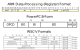
\includegraphics[width=\textwidth]{figures/formats}

\end{frame}

\begin{frame}[fragile]{Formats}

PowerPC B-Form

\begin{lstlisting}
"%opcd:6 %bo:5 %bi:5 %bd:14 %aa:1 %lk:1";
\end{lstlisting}

\bigskip

RISC-V R-Type

\begin{lstlisting}
"%funct7:7 %rs2:5 %rs1:5 %funct3:3 %rd:5 %opcode:7";
\end{lstlisting}

\end{frame}

\begin{frame}{Instructions}
\end{frame}

\begin{frame}{Decoding}

Elaborate example from before

\end{frame}

\begin{frame}{Branch Metadata}

% DBT systems can take advantage

% Can't easily tell if an instruction is a jump
% - would need to detect writes to PC register
% - could be aliased with a bank

\end{frame}
